\section{Early Science Data Products}
\label{sec:data}

All Rubin Observatory LSST data products are produced by the LSST Science Pipelines \cite{2019ASPC..523..521B,2018PASJ...70S...5B}.
For an introduction to the Rubin data products, see \citet{RubinDataProductsAbridged}.
Here we provide a summary of the data products that are expected to be made available as part of the \esp.

Each pre-operations data preview and survey data release will be accompanied by its own release-specific DPDD, giving e.g. the  database schema for the catalogs included in that dataset.
For an example data release DPDD, see the online DP0.2 documentation.\footnote{\url{https://dp0-2.lsst.io/data-products-dp0-2/}}

The Rubin data rights policy is described in  \cite{RDO-013}.

\subsection{Prompt data products}

Data products for transients, variable, and moving objects will be primarily produced by the Prompt Processing pipelines, which will perform reduction, calibration, difference image analysis (DIA), source detection and measurement, and alert distribution within 60 seconds of image readout.
They include images, catalogs and alerts.

During routine LSST operations, prompt image data products will be made available 80 hours following camera readout.
They include raw images, processed single visit images (PVIs), difference images, and template images.
Access to unvetted PVIs and difference images in the first 6 months of the LSST is still to be decided.
Prompt image products are proprietary, except for the alert postage stamps distributed in the alert stream and recorded in the alert database.
The image differencing source (\DIASource), forced photometry (\DIAForcedSource), and object (\DIAObject and \SSObject)
catalog data products are all public and will be available after 24 hours.
Rubin Data Rights holders can access both prompt image and catalog data products via the Rubin Science Platform (\S~\ref{ssec:dataaccess}) and query using VO interfaces.

Alerts are triggered by sources detected with SNR>5 via difference image analysis (DIA) and transmitted to community alert brokers for the list of selected brokers.
Alert packets transmitted to these brokers are world-public.
Similarly, daily Solar System Processing identifies new Solar System Objects from difference image sources and reports those publicly to the Minor Planet Center.

Alert production will begin shortly after System First Light, initially at low latency and limited volume but with both ramping up continuously through commissioning and into the first year of the survey.
In this way, Alert production and distribution is decoupled from the Data Preview schedule.

In the tables below, we indicate what kind of Alert stream can be expected during each data preview ``era,'' defined as the time period within which that data preview's images are obtained.
Note that the DP1 era is {\it very short}: the data products released in DP1 will be generated from relatively few observations taken in the few days around System First Light.
As such, it may not make much sense to run the Prompt Processing pipeline on the DP1 images.
Instead, the DP2 observations (commissioning's ``system optimization'' and Science Validation surveys) will be able to support prompt processing and alert generation shortly after System First Light.
DRP image differencing on the First Light image time series will enable some limited initial time domain science with DP1. 

\subsection{Data Release data products}

Static science datasets for Early Science will flow from the \svs in commissioning.
Images and catalogs from the DRP of the commissioning data will be made available to data rights holders in the form of Data Previews via the access mechanisms described in \S~\ref{ssec:dataaccess}.
Due to the relatively short time periods available for commissioning observations (\S~\ref{ssec:scenarios}), these Data Previews will necessarily be limited in their area and temporal coverage relative to full Data Releases, however all Data Preview data products will be in the same science data model format as for future Data Releases.


\subsection{Access to \es data products}\label{ssec:dataaccess}
Alerts will be accessible by the community via one or more of the nine Rubin-endorsed Community Brokers\footnote{See \url{https://www.lsst.org/scientists/alert-brokers}}.
The Rubin Data Rights community will access the Rubin data products via the Rubin Science Platform, \citep{LSE-319}.

\subsection{Summary of expected \es data products}

The tables in this section outline which data products can be expected in each \es data preview and data release, and when.

\begin{table}
\caption{Summary of data products expected in each data preview and early survey data release, as of December 2022.
In the case of DP1, these expectations come with considerable uncertainty: see Table~\ref{tab:dp-one-products} for more on this.}
\label{tab:summary}
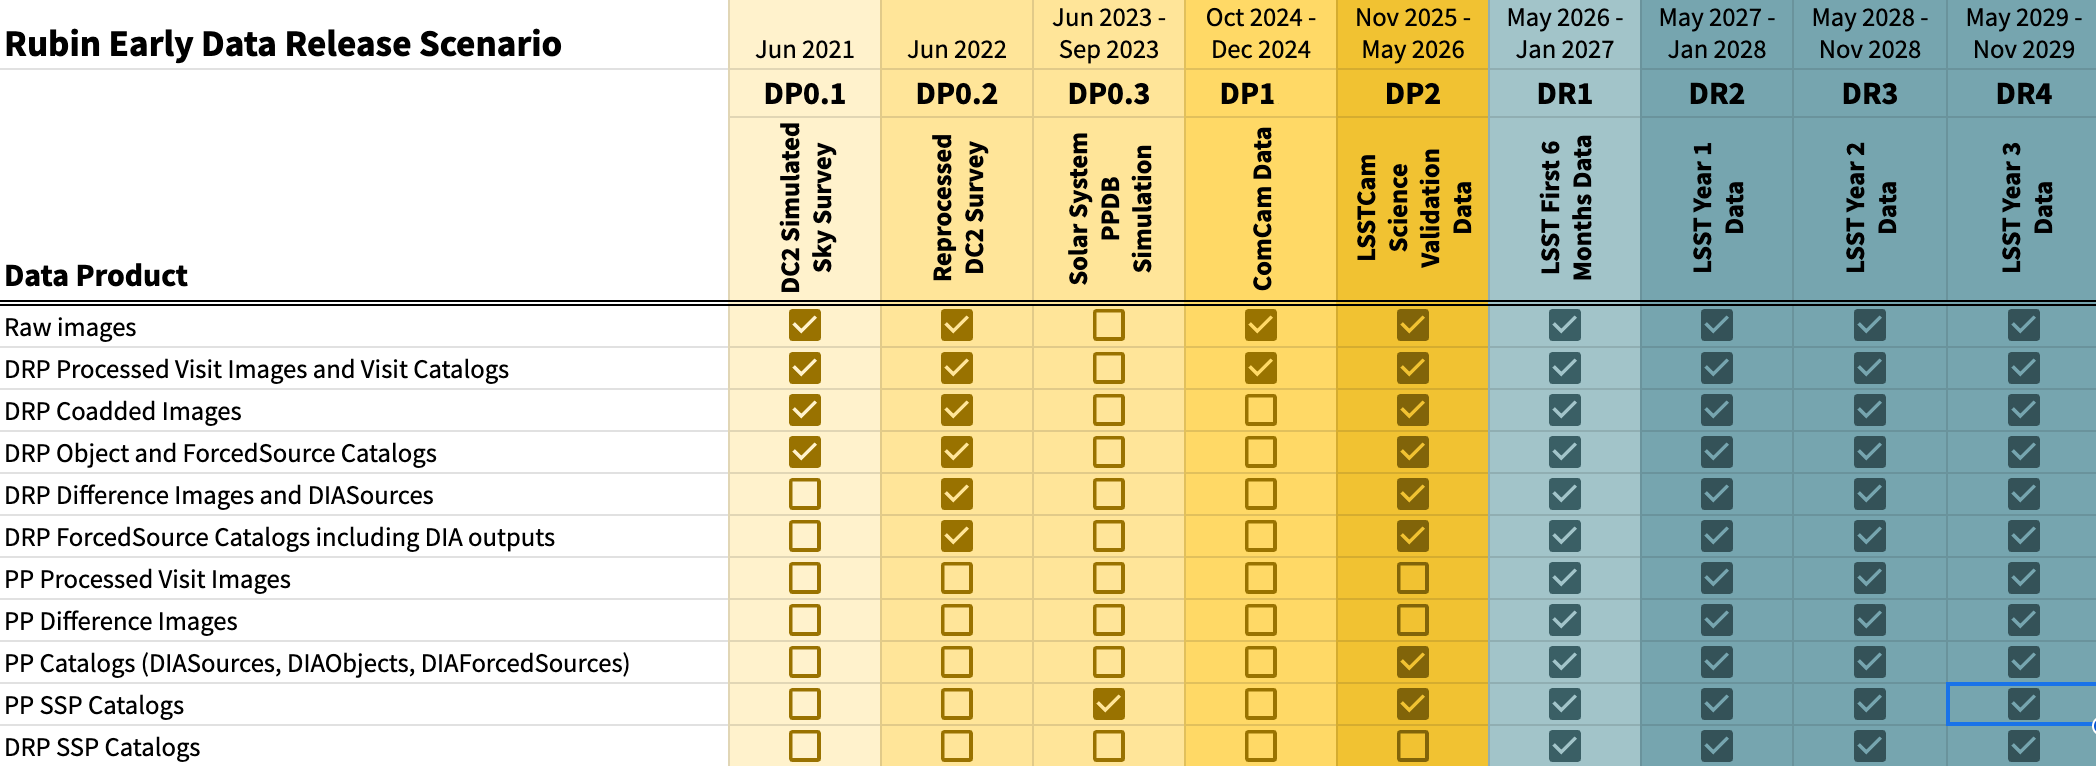
\includegraphics[width=\linewidth]{figures/DPR-summary}
\end{table}

\begin{table}
\caption{Summary of data products expected in DP1, as of December 2022.
Note the high degree of uncertainty in this table: DP1 will be planned in detail during 2023.}
\label{tab:dp-one-products}
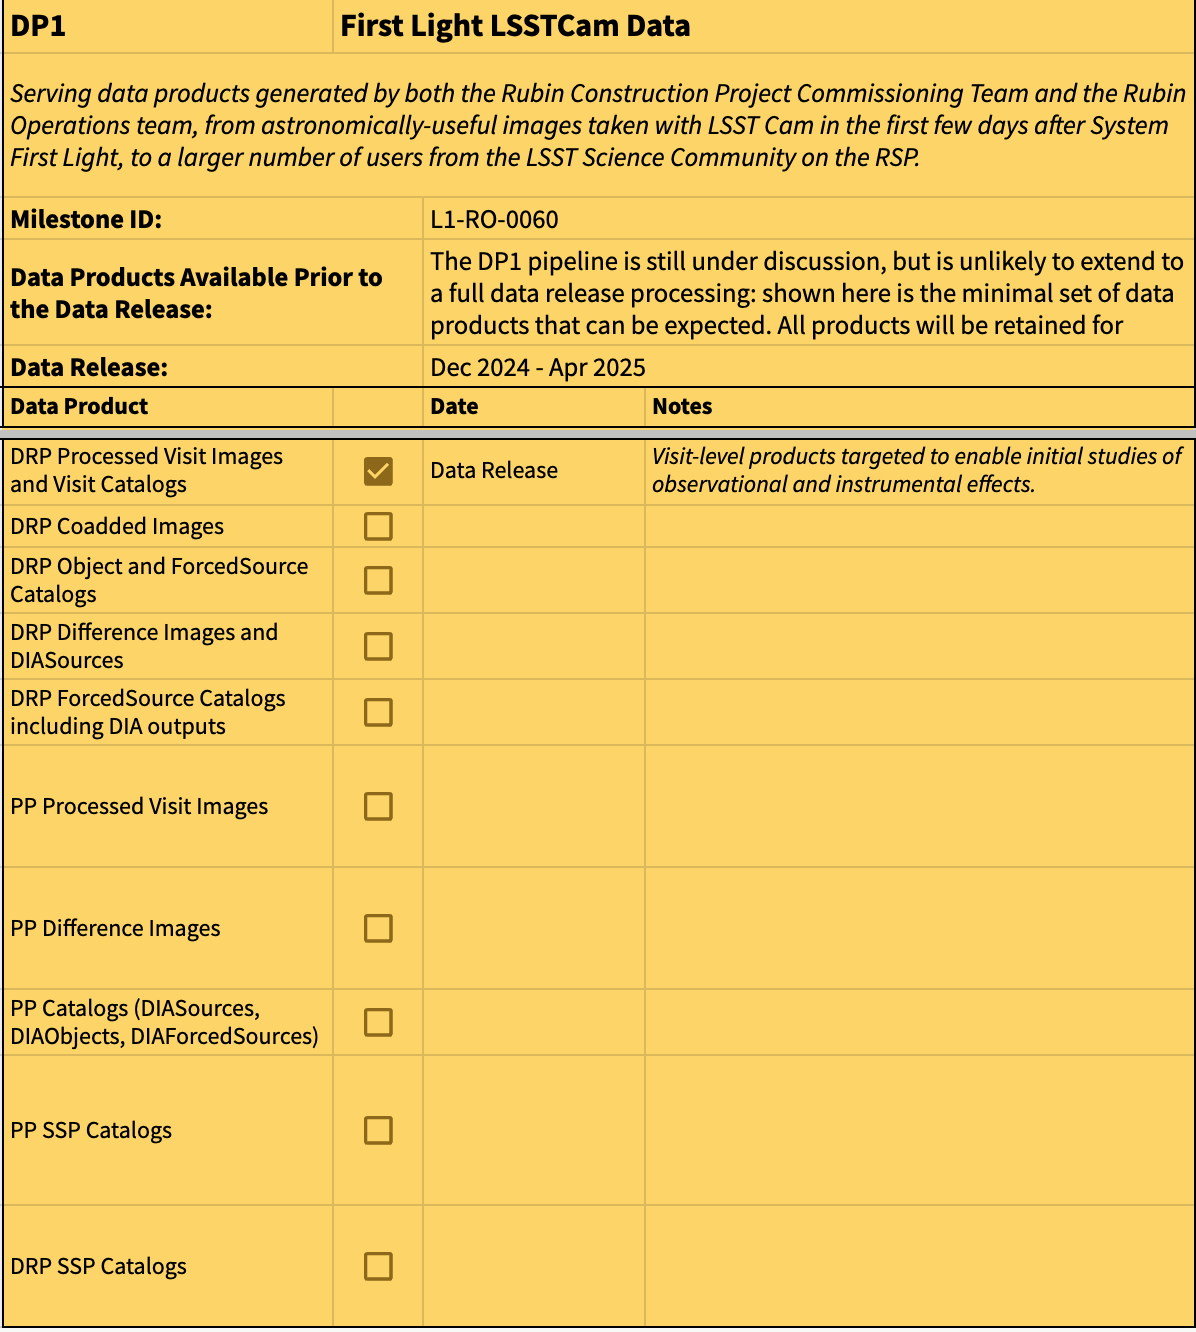
\includegraphics[width=\linewidth]{figures/DP1-products}
\end{table}

\begin{table}
\caption{Summary of data products expected in DP2, as of December 2022.}
\label{tab:dp-two-products}
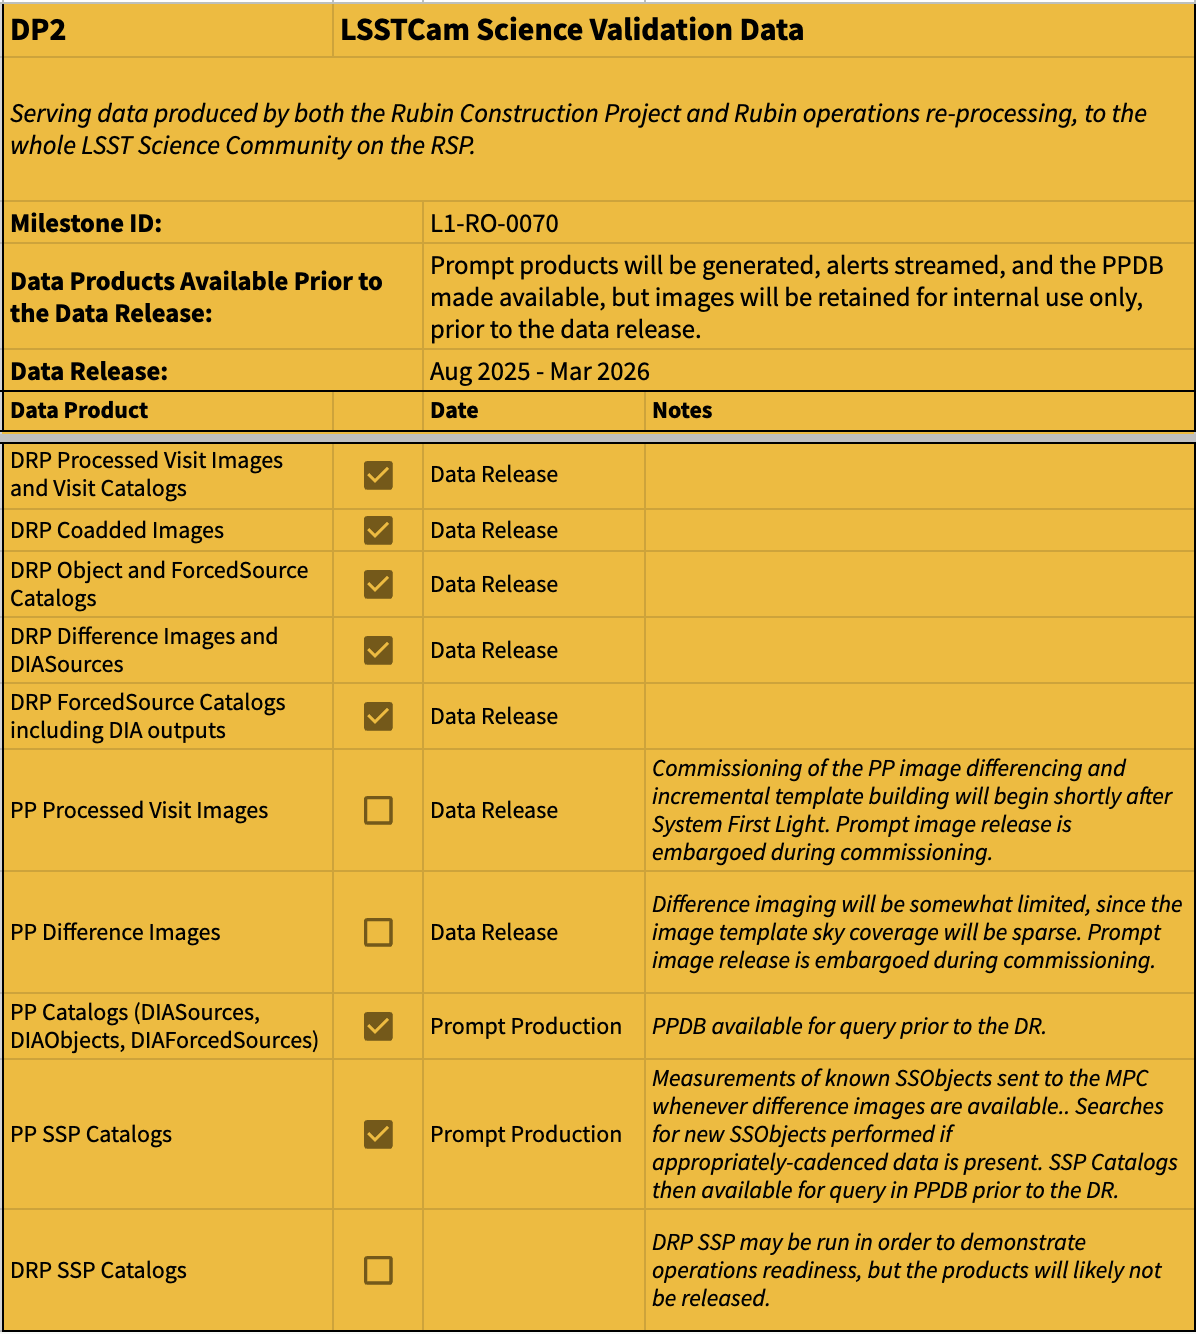
\includegraphics[width=\linewidth]{figures/DP2-products}
\end{table}

\begin{table}
\caption{Summary of data products expected in DR1, as of December 2022.}
\label{tab:dr-one-products}
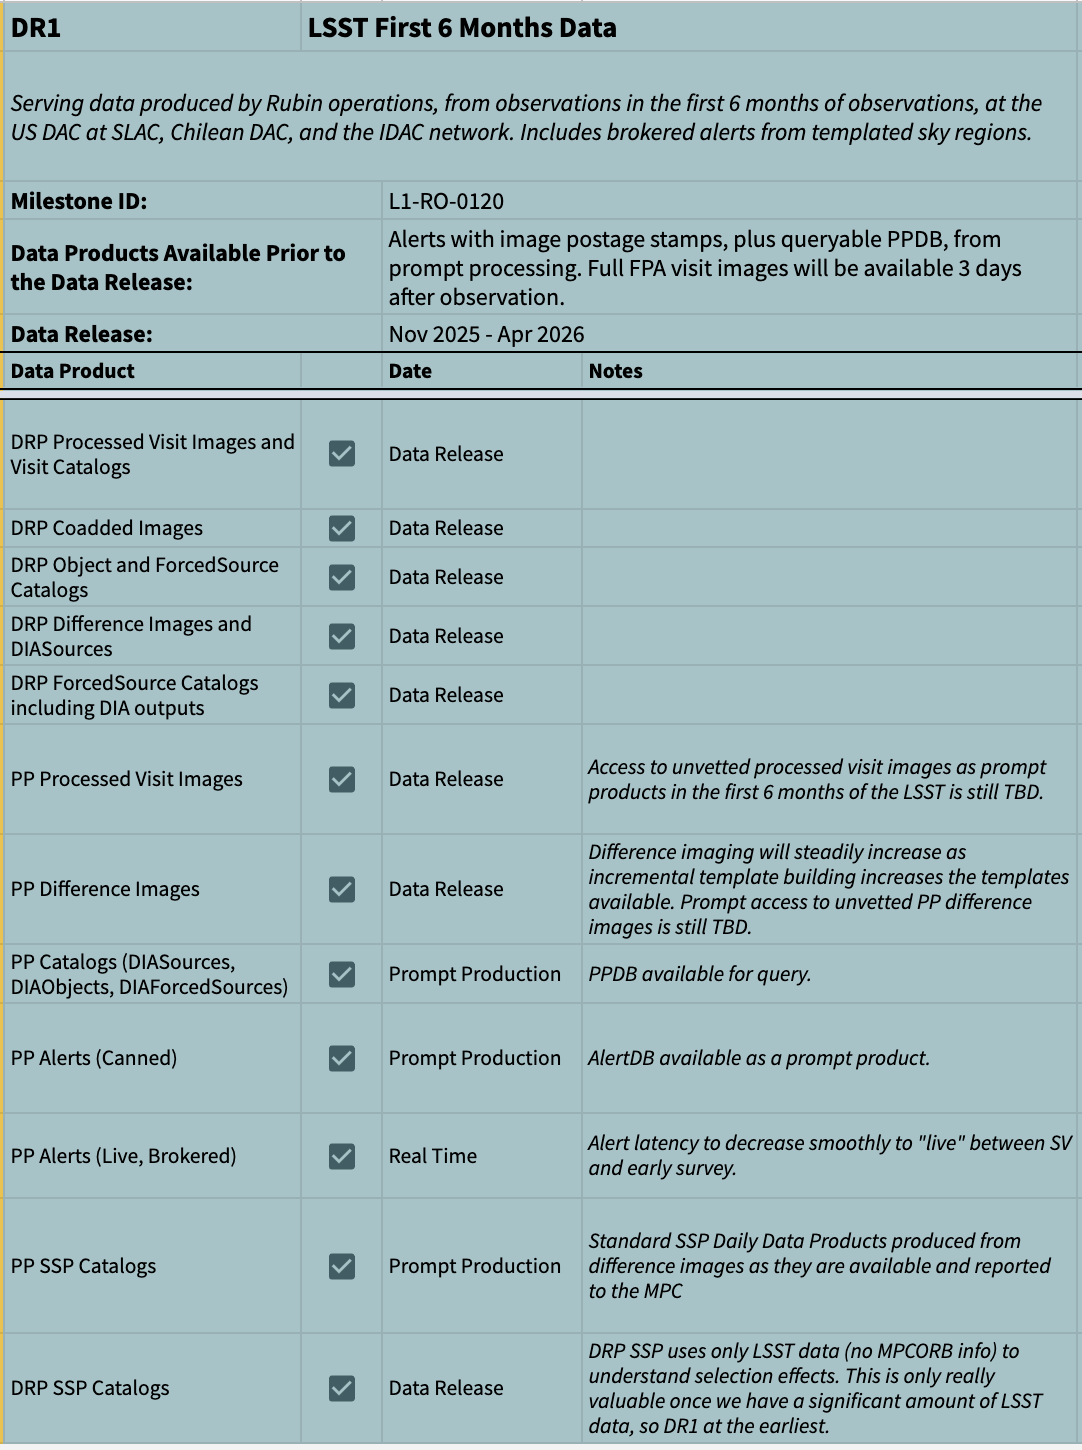
\includegraphics[width=\linewidth]{figures/DR1-products}
\end{table}
